\documentclass[10pt]{article}

%This is the minimal setup required to render the flag
\usepackage[paperwidth=120cm, paperheight=60cm, top=0cm, bottom=0cm, left=0cm, right=0cm]{geometry}
%Paper width is set to 120cm by 60 cm to match the Australian Government-specified aspect ratio (2:1)
\usepackage{tikz}
%\usepackage[dvipsnames]{xcolor} % Optional unless you want to use colors pre-defined by the xcolor package

% Australian Government-specified colors for the flag
\definecolor{aured}{RGB}{255,0,0}
\definecolor{auwhite}{RGB}{255,255,255}
\definecolor{aublue}{RGB}{0,0,139}

% Other government specifications include:
%Outer radius of Commonwealth star (below Union Jack) is 3/20 flag width, here it is 9 cm
%Outer radius of Alpha Crucis, Beta Crucis, Gamma Crucis and Delta Crucis is 1/14 flag width, here it is 30/7 cm
%Outer radius of Epsilon Crucis (5-point star) is 1/24 flag width, here it is 5/2 cm (2.5 cm)
%Inner radius of each star is 4/9 outer radius
%Positions from lower-left corner of flag:
%Center of Commonwealth star is 1/4 across and 1/4 up
%Center of Alpha Crucis is 3/4 across and 1/6 up
%Center of Beta Crucis is 5/8 across and 9/16 up
%Center of Gamma Crucis is 3/4 across and 5/6 up
%Center of Delta Crucis is 31/36 across and 151/240 up
%Center of Epsilon Crucis is 4/5 across and 11/24 up

%Source:
%http://www8.austlii.edu.au/cgi-bin/viewdoc/au/legis/cth/consol_act/fa195361/sch1.html

%Created by Senan Sekhon, December 24, 2020

\begin{document}

\begin{center}
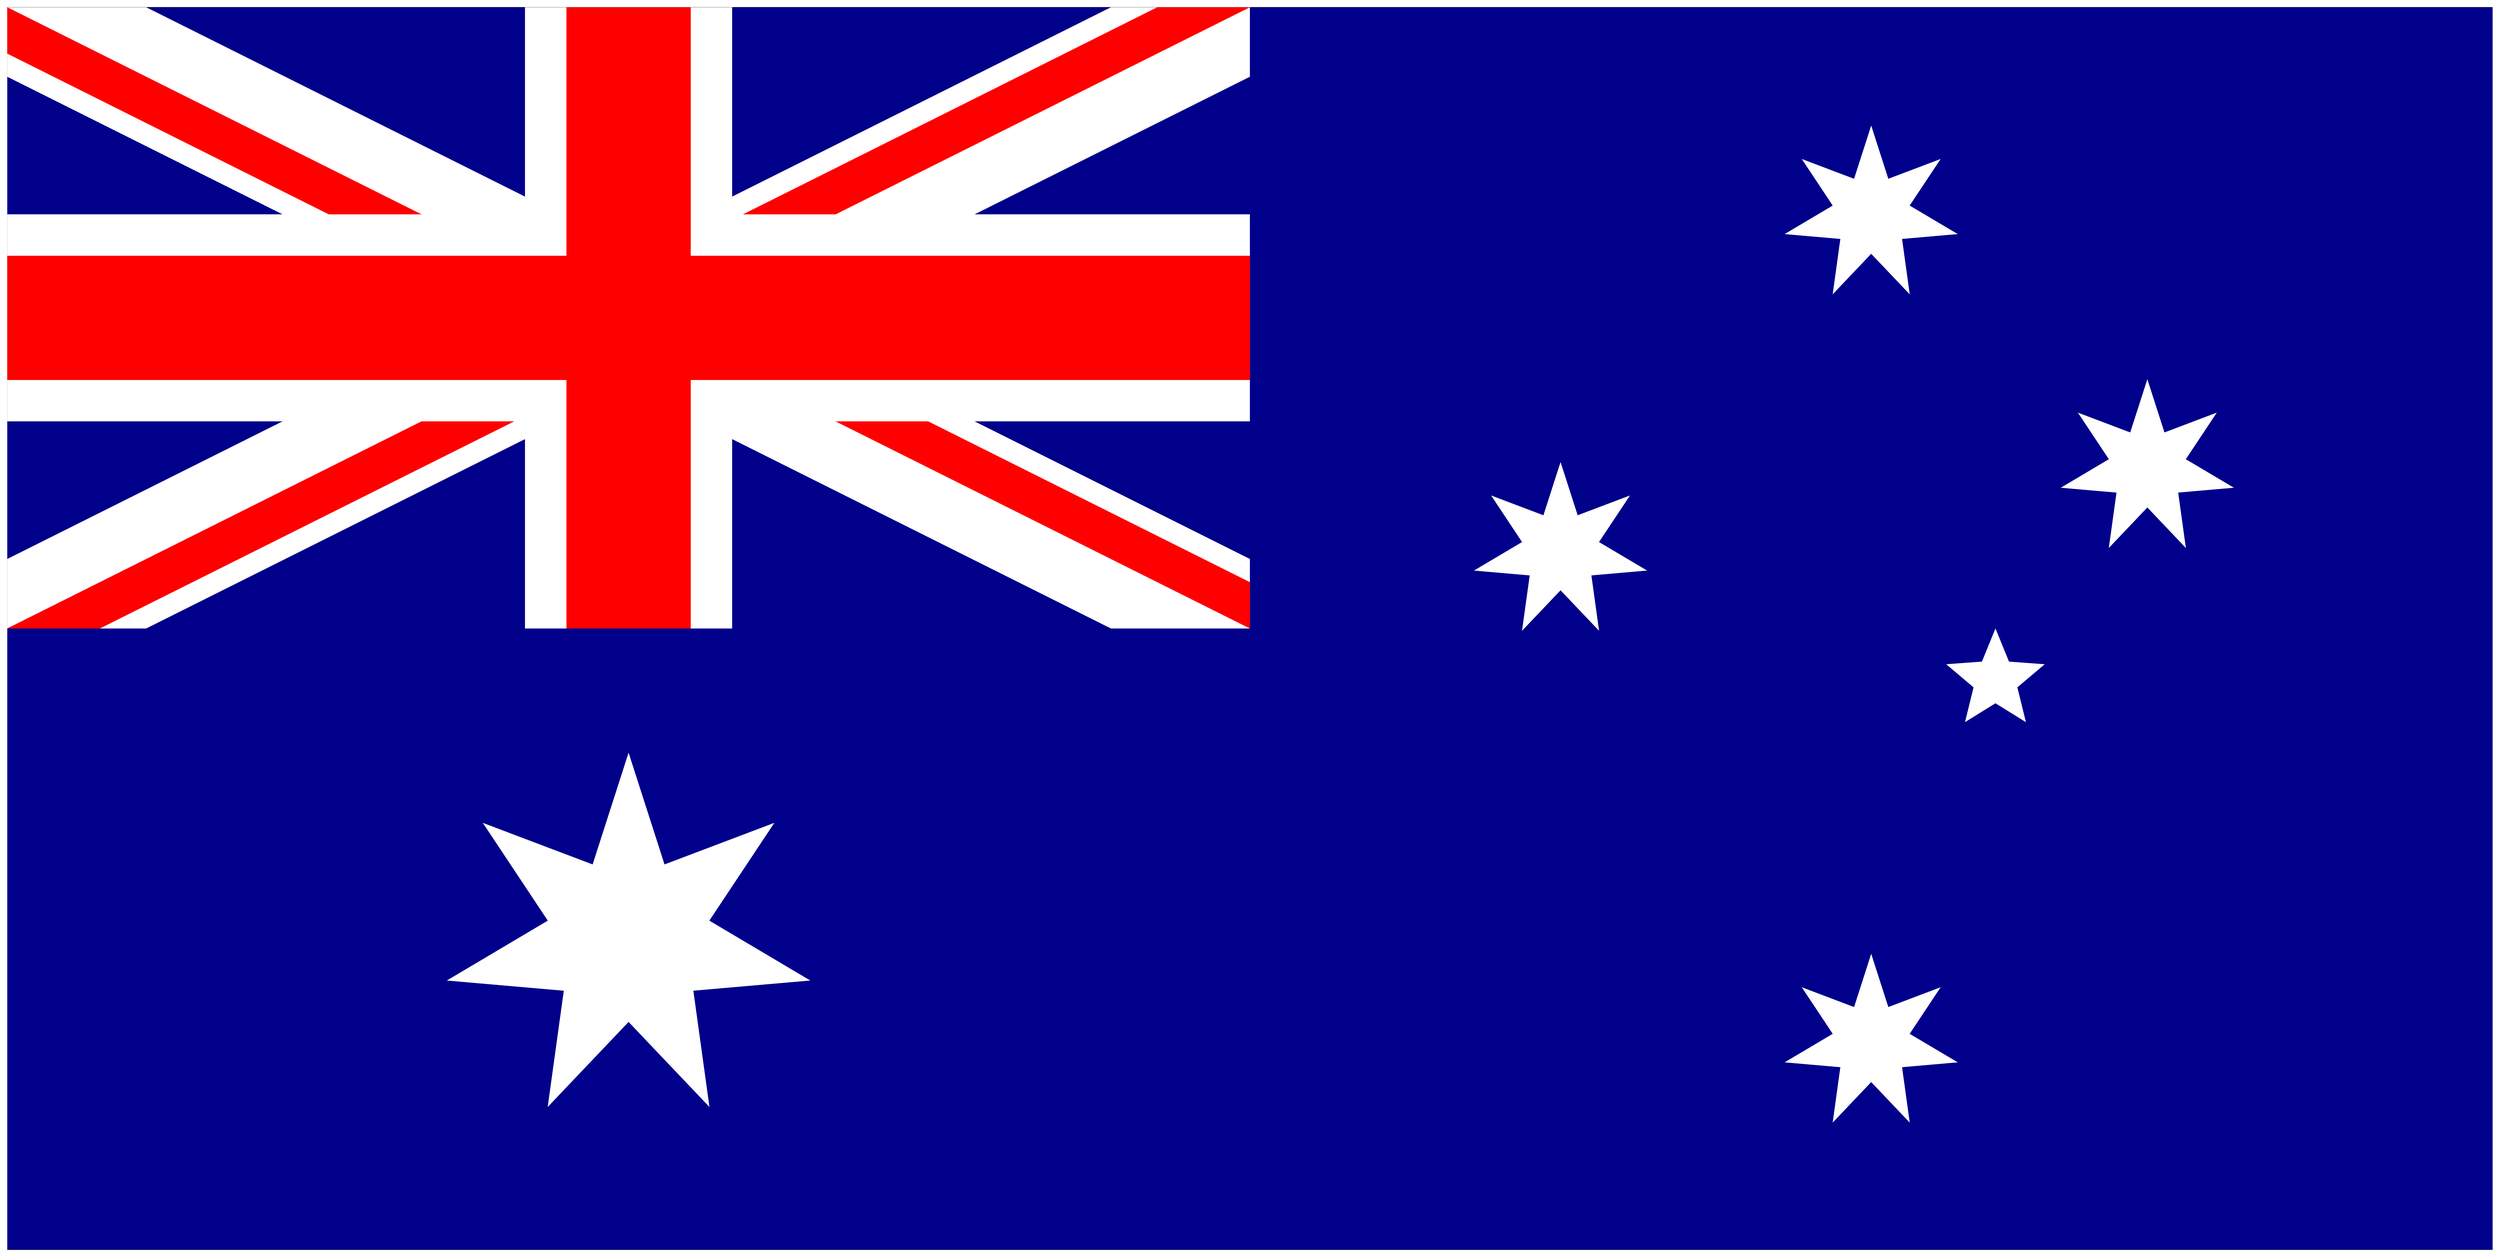
\begin{tikzpicture}[scale=1] %Scale must be changed to make the flag fit on letter/A4 paper (scale=1 produces a 120 cm by 60 cm flag)
\clip (-60,-30) rectangle (60,30); %Optional, crops the flag to the correct size
\draw[-] (-60,-30)--(60,-30)--(60,30)--(-60,30)--cycle; %Optional, draws a border around the flag
\fill[aublue] (-60,-30)--(60,-30)--(60,30)--(-60,30)--cycle; %Blue background
%Union Jack at the upper-left corner of the flag (with auwhite and aured colors and without blue background)
%Taken from https://www.overleaf.com/latex/examples/flag-of-the-united-kingdom/xcxqkwpvnxbs
\begin{scope}[shift={(-30,15)},scale=1,rotate=0]
%White upright cross:
\fill[auwhite] (5,15)--(5,5)--(30,5)--(30,-5)--(5,-5)--(5,-15)--(-5,-15)--(-5,-5)--(-30,-5)--(-30,5)--(-30,5)--(-5,5)--(-5,15)--cycle;
%White St. Andrew's Cross:
\fill[auwhite] (-30,-15)--(-30,{-15+3/2*sqrt(5)})--({30-3*sqrt(5)},15)--(30,15)--(30,{15-3/2*sqrt(5)})--({-30+3*sqrt(5)},-15)--cycle; %Lower-left to upper-right
\fill[auwhite] (-30,15)--(-30,{15-3/2*sqrt(5)})--({30-3*sqrt(5)},-15)--(30,-15)--(30,{-15+3/2*sqrt(5)})--({-30+3*sqrt(5)},15)--cycle; %Upper-left to lower-right
%Red upright Cross:
\fill[aured] (3,15)--(3,3)--(30,3)--(30,-3)--(3,-3)--(3,-15)--(-3,-15)--(-3,-3)--(-30,-3)--(-30,3)--(-30,3)--(-3,3)--(-3,15)--cycle;
%Red St. Patrick's Cross:
\fill[aured] ({10-2*sqrt(5)},5)--(10,5)--(30,15)--({30-2*sqrt(5)},15)--cycle; %Upper-right diagonal
\fill[aured] (-10,5)--({-10-2*sqrt(5)},5)--(-30,{15-sqrt(5)})--(-30,15)--cycle; %Upper-left diagonal
\fill[aured] ({-10+2*sqrt(5)},-5)--(-10,-5)--(-30,-15)--({-30+2*sqrt(5)},-15)--cycle; %Lower-left diagonal
\fill[aured] (10,-5)--({10+2*sqrt(5)},-5)--(30,{-15+sqrt(5)})--(30,-15)--cycle; %Lower-right diagonal
\end{scope}

%Template for a 5-point star, this can be shifted, scaled and rotated as you wish (inner radius is fixed at 4/9 outer radius)
\def\star{(0,1)--({4/9*cos(54)},{4/9*sin(54)})--({cos(18)},{sin(18)})--({4/9*cos(18)},{-4/9*sin(18)})--({cos(54)},{-sin(54)})--(0,-4/9)--({-cos(54)},{-sin(54)})--({-4/9*cos(18)},{-4/9*sin(18)})--({-cos(18)},{sin(18)})--({-4/9*cos(54)},{4/9*sin(54)})--cycle}
%Template for a 7-point star, this can be shifted, scaled and rotated as you wish (inner radius is fixed at 4/9 outer radius)
\def\sstar{(0,1)--({4/9*cos(450/7)},{4/9*sin(450/7)})--({cos(270/7)},{sin(270/7)})--({4/9*cos(90/7)},{4/9*sin(90/7)})--({cos(90/7)},{-sin(90/7)})--({4/9*cos(270/7)},{-4/9*sin(270/7)})--({cos(450/7)},{-sin(450/7)})--(0,-4/9)--({-cos(450/7)},{-sin(450/7)})--({-4/9*cos(270/7)},{-4/9*sin(270/7)})--({-cos(90/7)},{-sin(90/7)})--({-4/9*cos(90/7)},{4/9*sin(90/7)})--({-cos(270/7)},{sin(270/7)})--({-4/9*cos(450/7)},{4/9*sin(450/7)})--cycle}

\begin{scope}[shift={(-30,-15)},scale=9,rotate=0]
\fill[auwhite] \sstar; %Commonwealth star
\end{scope}

%Outer scope for shifting, scaling and rotation of the entire Southern Cross
\begin{scope}[shift={(30,0)},scale=1,rotate=0]
%Inner scopes for shifting, scaling and rotation of each individual star
\begin{scope}[shift={(0,-20)},scale=30/7,rotate=0]
\fill[auwhite] \sstar; %Alpha Crucis
\end{scope}
\begin{scope}[shift={(-15,15/4)},scale=30/7,rotate=0]
\fill[auwhite] \sstar; %Beta Crucis
\end{scope}
\begin{scope}[shift={(0,20)},scale=30/7,rotate=0]
\fill[auwhite] \sstar; %Gamma Crucis
\end{scope}
\begin{scope}[shift={(40/3,31/4)},scale=30/7,rotate=0]
\fill[auwhite] \sstar; %Delta Crucis
\end{scope}
\begin{scope}[shift={(6,-5/2)},scale=5/2,rotate=0]
\fill[auwhite] \star; %Epsilon Crucis (5-point star)
\end{scope}
\end{scope}
\end{tikzpicture}
\end{center}

\end{document}